\section{Market for a Sea of XPU's are the \emph{closed} hyperscalars}

\begin{figure}
  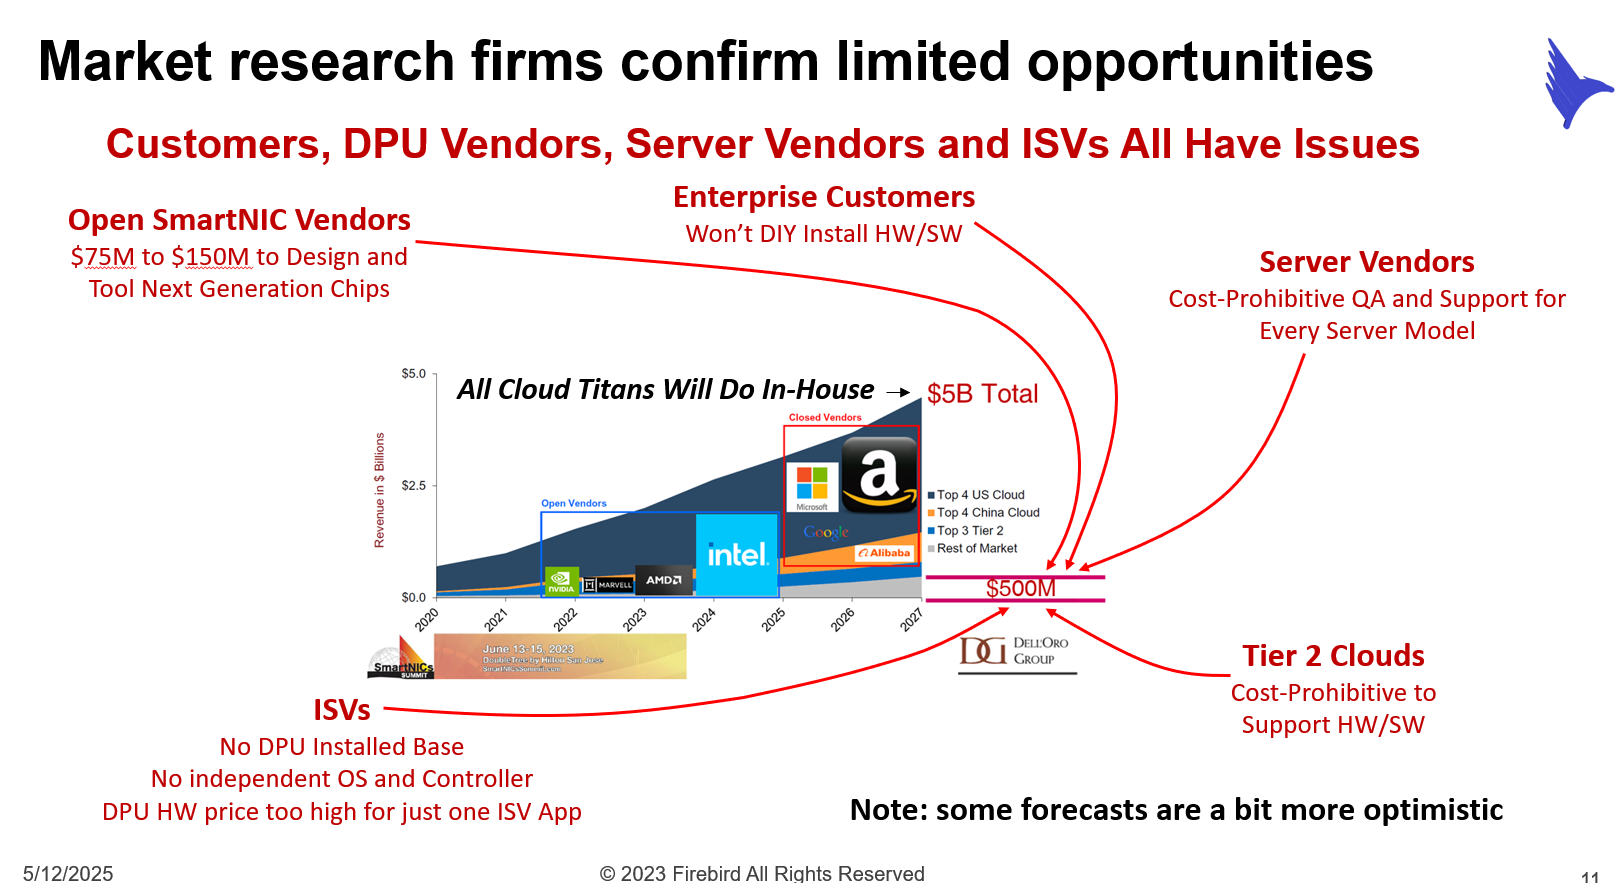
\includegraphics[width=\linewidth]{../../FIGURES/XPU-market.png}
  \caption{The SmartNIC Revolution died, long live the XPU Revolution. Courtesy: Harry V. Quackenboss}
\end{figure}

 
The FPGA NICs aren’t cheap compared to a standard NIC.  The only ones our use cases would work with were RISC-based Linux ones with, if not currently, at least planned, per-core (single-thread) performance close to single-thread performance of a Xeon core. Broadcom’s Stingray II (shelved), Marvell’s high-end Arm processor (never produced in volume), and Intel’s Mt. Evans roadmap (never pursued for anybody other than hyperscalers).  NVIDIA’s BlueField 4 (not yet released – maybe shelved) looked good on paper.
 
The really high-volume prices of the SmartNICs in the BlueField-3 class were probably as low as \$700 per unit, which I suspect is still less way than FPGA NICs.
 
For our use cases, price/performance was better on these types of SmartNICs because the data in flight nature of the workloads meant less DRAM/core, and the RISC versus X86 advantage of ~70\% in MIPS/Watt meant it made sense to offload those. However, if the SmartNICs couldn’t keep up with he geometry shrink from 3nm -> 2nm and so on that the CPUs were on, the per-core performance and MIPS/Watt advantage evaporated.
 
 --------------
Harry Quackenboss


\bigskip
\newpage
 
Are these honking big, expensive smart NICs you're talking about?  I think we can implement our protocol in a pretty simple FPGA.  (It can be really simple if we do failure recovery with the CPU.)  In fact, there was an FPGA implementation.  John Lockwood may know the details.
 
Years ago we spoke to a NIC vendor.  We could implement 99\% of the protocol with small changes to their standard product.  There was one corner case that required a change to their pico-code that was the showstopper for them.  None of those changes would have been visible to customers not using our protocol.

--------------
Alan Karp
 
\bigskip

%==========

I'd say the future is highly interconnected processors that have specialized computing support, SmartNICs fall in the specialized computing category if they have engines for things like encryption and compression, or something general purpose like an FPGA.

--------------
Kev.

\bigskip

%On Mon, May 12, 2025 at 11:16 AM Alan Karp via groups.io <alanhkarp=gmail.com@groups.io> wrote:
Thanks for this perspective.  I had thought that smart NICs everywhere was the wave of the future.

That being said, I'm not sure we need smart NICs for the basic protocol.  I believe that the happy path can be handled by simple state machine logic in the NIC.  Recovery from a broken link or node is probably too complex for that, so it would have to be handled by the CPU.  Recovery would certainly take longer, perhaps ms instead of microseconds.

--------------
Alan Karp


%On Fri, May 9, 2025 at 5:18 PM Harry V. Quackenboss via groups.io <harry=quackenboss.com@groups.io> wrote:
It strikes me that among Kevin, Alan, and Hesham, there is no common understanding of what the minimum NIC feature set is that this future protocol suite would run on  (or, for that matter, possible middle boxes such as L2 switches)

Adrian is current on this stuff, and I am not, but my understanding is that SmartNICs, to summarize, are used by AWS, Google, Microsoft, and Meta (and as a first approximation, Meta is less than 1/5 the size of the others), but each vendor controls the SW stack including host drivers, and firmware on the SmartNIC, and even at least some HW features. And, at least for now, none of the public cloud subset is making programmability available to customers.

I don’t see how this effort is going to impact that, but maybe Adrian has a different opinion.

Other than niches (and compared to markets big enough to support new silicon at the rate CPUs evolve, even FPGA NICs are in my taxonomy, niches). NVIDIA’s adaption of their DPU family to allow tuning for RDMA in AI and HPC clusters (that NVIDIA calls “SuperNIC”) isn’t really an exception in my view.  There isn’t a significant installed base. If you scrutinize the forecasts and separate out vendors obfuscating to situation by declaring their high-end server NICs as SmartNICs, none are forecast big growth in the future (again, excluding hyperscalers).

A conclusion I draw from that is that trying to create new broad industry standards is inconsistent with depending on hardware roadmaps for NIC features that aren’t forecast to be big volumes (excluding the hyperscalers that are going to be difficult to influence.

Translation: if this effort depends on custom programmable NICs (SmartNICs) isn’t going to lead to broad interest.

The sooner this group can come to a common understanding about whether SmartNICs are in or out of scope, the sooner the debate can be narrowed.

I personally would love to see SmartNICs be widely adopted. As Kevin intimates, there are a bunch of things one can do.

I just think unless and until factors beyond this group’s ability to influence change, it’s like trying to start a campfire with damp kindling in the rain. Smoke, with effort. But not much fire.


\bigskip
% 
--------------
Harry
